\gobbletocpage
\chapter{Improvements of Ecotype Simulation}
\restoretocpage
%\begin{shadequote}
%\begin{center}
%    \Large\begin{verbatim} 
%        Harder, Better, Faster, Stronger
% \end{verbatim}  
%\end{center}
%\par--\emph{Daft Punk}
%\end{shadequote}

\begin{shadequote}
\begin{center}
    \Large\begin{verbatim} 
             Citius, Altius, Fortius
 \end{verbatim}  
\end{center}
\par--\emph{Olympic Motto}
\end{shadequote}
%%Faster, Higher, Stronger


\section{Improvements}
ES1 set hard input size limits of two thousand sample sequences of at most three thousand nucleotides~\cite{koeppel2008identifying}.
However, I doubt it was ever run with even close to that many sequences.
When run on input sizes of greater than only one hundred sequences time became a limiting factor.
Previous work showed that while ES1 had superior \index{demarcation} accuracy to its contemporaries, ES1 could not compete in run-time comparisons.
And as we increase the sample size running time increases dramatically.
See Table \ref{tab:ES1speed}.
This issue is clearly a priority for improvement.

To solve the problem we came up with two approaches.
First, modify the main ES algorithm driving the program.
Second, reorganize execution to take advantage of large computer clusters (parallelization).
I will focus mainly on modifications to the ES algorithm, which are prominently featured in ES2, and briefly address my colleague, Lingyuan Ke's, approach to (parallelization) which will be featured in future Ecotype Simulation iterations.
Finally, I will discuss future plans for improving the Ecotype Simulation software family.


\subsection*{Ecotype Simulation 2.0}
This is the version of ES I thoroughly test in chapter four in comparison to other demarcating programs.
While the changes are few in number, we believe that they will increase the practicality of using ES approach to understanding microbial diversity.

\begin{table}
 %\begin{tabular}{| l | l | l | l |}
 \begin{tabular}{| c | c | c | c |}
  \hline
  Algorithm & 20 sequences & 30 sequences & 50 sequences \\ \hline
  ES & 69.8 & 384 & 2390 \\
  AdaptML & 1.54 & 1.57 & 1.64 \\
  GMYC & 0.201 & 0.292 & 0.549 \\
  BAPS & 4.80 & 5.15 & 6.12 \\
  \hline
 \end{tabular}
 \caption[ES1 run-time compared to other demarcation programs.]{The run speed is measured in seconds (reprinted from \protect\cite{carlo})}
 \label{tab:ES1speed}
\end{table}

\subsubsection*{Key algorithmic changes}
Backwards and forward simulation takes up most of ES1 run time.
The simulation process is called many times throughout the entire typical program execution.
If we can come up with a way to reduce the time complexity of simulations, great speed improvements are possible.

For ES2 we run the backwards simulation of node coalescence exactly the same.
However, once we have the evolutionary history scaffold we can use properties of ultra-metric phylogenetic trees.
Ultra-metric trees have the same distance between root to tip for all organisms, and usually are made under the assumptions of a deterministic rather than a stochastic molecular clock~\cite{ho2008molecular}.
By the length between two nodes we can determine time between organisms.
Based on this fact performing binning is unnecessary.
ES2 can conduct a linear pass through the backwards scaffold directly comparing it to the observed sequence identity graph, checking for success and failure with all precision levels.
This insight removes an $O(n^3)$ factor, immediately quickening the algorithm. [Perhaps go into more detail?]

\subsubsection*{Demarcation}
In addition to core algorithm changes we made changes to the auto-demarcating program.
Instead of demarcation confidence intervals, ES2 runs the downhill-simplex (Hillclimbing) method on each subtree as we recursively descend through the phylogeny.
Normally our Bruteforce method must be run before Hillclimbing, in this case we use results from Hillclimbing as a seed for the closest ancestor node.
Then at each child node we use Hillclimbing results from the parent node, bypassing running Bruteforce for each subtree.
This maintains a high level of accuracy without compromising speed.

%THINK ABOUT HOW TO ORDER THIS SECTION AND MAKE HEADERS
\section{Future Improvements}
Through the work involved with this project we realized that in addition to speed, space has become a limiting factor.
To make a distance divergence matrix we need $O(n^2)$ space, and with number of sequences in the thousands we quickly run out of RAM. Also, the current implementation has similar time complexity to the naive $O(n^3)$ approach.
We explored different clustering packages that had various space and time trade-off balances.

Besides improving our clustering technique, parallelizing the ES algorithm is the highest priority.
I will briefly overview our designs and results in parallelizing ES.
However, the reader should refer to, my colleague, Lingyuan Ke's senior thesis for full details.
%\subsection*{Ecotype Simulation 3.0}
\subsection*{Binning}
As mentioned in previous sections ES uses complete linkage clustering.
The current implementation is in Fortran90, and we have yet to update it to reflect improvements in the state of the art.
Big Data companies have developed an interest in clustering large datasets, resulting in various improvements in clustering algorithms.
\subsubsection*{Current implementation}
%First I'll go over our naive implementation here
Our naive approach is as follows:
%FROM WIKIPEDIA!  CITE!
\begin{enumerate}[I]
\item Begin with the disjoint clustering having level $L(0) = 0$ and sequence number $m = 0$.
\item Find the most similar pair of clusters in the current clustering, say pair $(r)$, $(s)$, according to $d[(r),(s)] = max$ $d[(i),(j)]$ where the maximum is over all pairs of clusters in the current clustering.
\item Increment the sequence number: $m = m + 1$. Merge clusters $(r)$ and $(s)$ into a single cluster to form the next clustering m. Set the level of this clustering to $L(m) = d[(r),(s)]$
\item Update the proximity matrix, $D$, by deleting the rows and columns corresponding to clusters $(r)$ and $(s)$ and adding a row and column corresponding to the newly formed cluster. The proximity between the new cluster, denoted $(r,s)$ and old cluster $(k)$ is defined as $d[(k), (r,s)] = max$ $d[(k),(r)]$, $d[(k),(s)]$.
\item If all objects are in one cluster, stop. Else, go to step II.
\end{enumerate}
which ends up running at $O(n^3)$ time (written up using~\cite{FastClust} as a reference).
In our case we divide the processing by first calculating a pairwise distance matrix between all sequences.
That way we maintain a look up table, $D$, to look up distance in constant time.
At each iteration two clusters are merged (specifically the closest by the specified distance function) and the divergence matrix is updated with a distance entry between each cluster and the new cluster (specifically the element of each cluster being compared that is the farthest apart).

\subsubsection*{State of the art}
From the literature we discovered that there are complete-linkage clustering implementations that achieve $O(n^2)$ time complexity.
We found fastcluster, a well-documented and tested C++ library that efficiently implements several hierarchical clustering algorithms~\cite{mullner2011modern, FastClust}.
The library includes complete-linkage clustering that runs in $O(n^2)$ (for a graphical comparison of various clustering package see Figure~\ref{fig:FastClustComparison}).

\begin{figure}[h!]
\centering
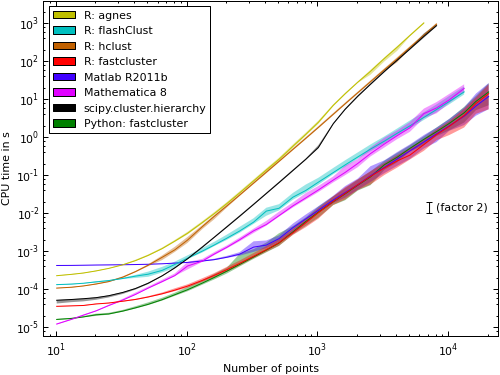
\includegraphics[scale=0.75]{images/FastComplete-CH3}
\caption[Complete linkage clustering speed comparison between popular implementations.]{The colored bands show maximum and minimum time over a variety of data sets. The average is plotted as a solid line. The synthetic data sets are samples drawn in an iid. manner from various mixtures of Gaussian distributions in Euclidean space of various dimensions.
%The results were obtained on a PC with an Intel dual-core CPU T7500 with 2.2 GHz clock speed and 4GB of RAM. The operating system was Ubuntu 11.04 64-bit (Ubuntu 10.04 64-bit for Matlab R2010a). R version: 2.13.0, fastcluster version: 1.1.7, flashClust version: 1.01, Python version: 2.7.1, NumPy version 1.5.1, SciPy version: 0.8.0.
(reprinted from \protect\cite{FastClust})}
\label{fig:FastClustComparison}
\end{figure}

I quickly linked up fastcluster to ES2, replacing our naive binning implementation and achieved impressive speed results (see Figure~\ref{fig:FastVsNaive}).

\begin{figure}[h!]
\centering
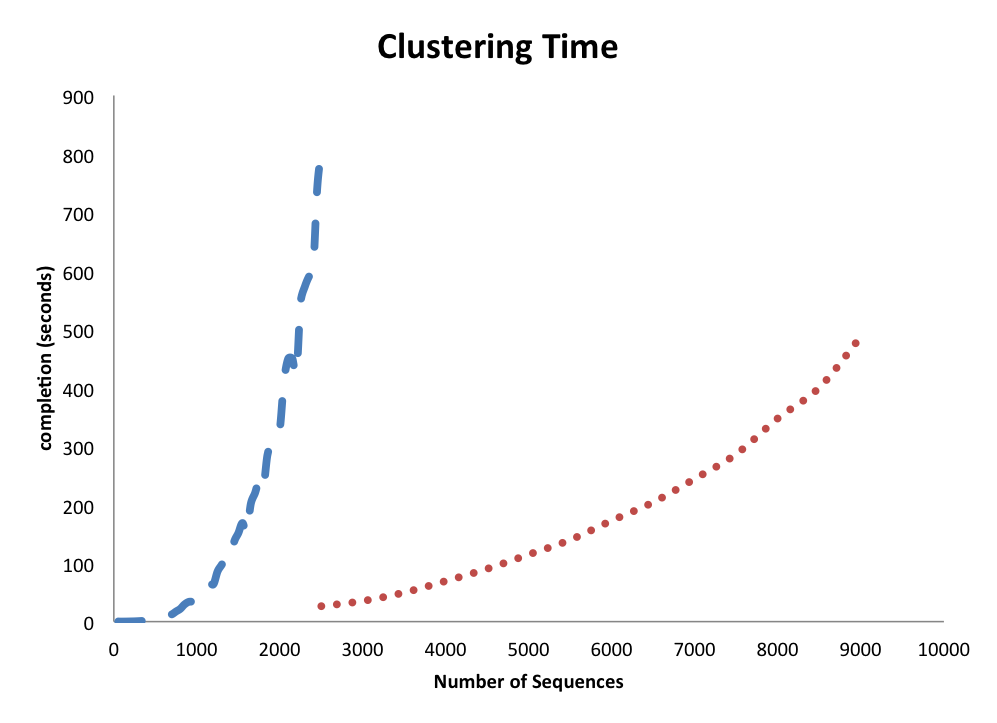
\includegraphics[scale=.8]{images/FastVsNaive-CH3}
\caption[Time comparison of fastcluster versus our naive implementation of complete-linkage clustering.]{Times comparison of fastcluster (red) versus our naive (blue) implementation of complete-linkage clustering. [REMOVE COLOR!]}
\label{fig:FastVsNaive}
\end{figure}

Our current implementation was not capable of clustering datasets of greater than approximately three thousand sequences.
On the other hand fastcluster handled files with more than fifteen thousand sequences, until memory on my machine became a factor.
As far as accuracy goes, each bin level was within one or two of the current implementation (the slight error might be attributable to my quick hack job) in preliminary tests.

However, many more tests are needed to insure the package will work correctly for our purposes and we are not enthusiastic about adding another dependency to ES.
For now it is an envisioned improvement for the next version.

\subsubsection*{Minimizing space usage}
%None of that matters if we can't decrease the space usage.
%Approach one, don't save a divergence matrix
%Here I could include some of my code.
While increasing speed efficiency is important, the bottleneck has increasingly become space usage.
Our goal is to run ES on up to one million sequences, which in our current approach would entail a million squared pairwise distance matrix ($n \times n$).

In one exploratory approach we attempted to fix this problem by skipping the distance matrix generating step altogether.
Instead, we could define a replacement function that will calculate the distance between clusters at runtime (see Figure~\ref{code:LazyClustering}).

%\begin{figure}[h!]
%\centering
%\noindent\code{Lazy Clustering}{code/lazy_formatted.py}
%\caption[Python code showing a distance function for two clusters.]{The two clusters are represented by $c1$ and $c2$, while $seqs$ is a list used to access strings of sequence. The function $seq$\_$distance$ takes two strings representing sequences and returns the manhattan or taxicab distance between them. This python function returns the distance between two clusters.}
%\label{code:LazyClustering}
%\end{figure}


\begin{figure}[h!]
\begin{algorithm}[H]
 \SetAlgoLined
% \KwData{c1 is a cluster of sequences, c2 is another cluster of sequences, seq-dist is a function that takes two sequences and returns the distance between them}
% \KwResult{the distance between two clusters}
\SetKwInOut{Input}{input}\SetKwInOut{Output}{output}

\Input{c1, c2 are different clusters of sequences}
\Output{The distance between two clusters, contained in $max$-$dist$}
\BlankLine
 $max$-$dist \gets 1.0$\\
 \For{$s1 \in c1$} {
   \For{$s2 \in c2$} {
    $d \gets seq$-$dist(s1, s2)$\\
    \If {$d < max$-$dist$} {
      $max$-$dist \gets d$
    }
   }
 }
\end{algorithm}
\caption[Pseudocode showing a distance function for two clusters.]{The two clusters are represented by $c1$ and $c2$, while $s1$ and $s2$ represent sequences in the clusters. The function $seq$-$dist$ takes two sequences and returns the manhattan or taxicab distance between them. This pseudocode returns the distance between two clusters.}
\label{code:LazyClustering}
\end{figure}


Clusters would start small, and then coalesce into larger clusters.
Thus the number of comparisons would remain relatively constant and there would be no distance matrix to store.
In this case, we would be choosing to minimize space usage, while greatly slowing down runtime.
It might be worth implementing a similar cluster distance function to use within the fastcluster complete-linkage implementation.
However, we would still hit a clustering time or space limit fairly quickly.

%Approach two, bin in parallel.
A second option for minimizing space usage and runtime would be to develop (or find in the literature) a complete-linkage clustering algorithm that could run in parallel.
This strategy is still in early development.
The difficulty would be in splitting up the sequences into discrete tasks that could then be combined after computation.
Each of those discrete tasks could be spread out in a cluster, reducing run time, or even run at different times, freeing up memory.

Either way, there is much progress to be made in Binning.
If ES is ever to work on one million sequences, Binning must be a major priority for future versions.

\subsection*{Demarcation}
The current auto demarcation program has a serious problem with paraphyletic groups.
Instead of maintaining a species group when one of the organisms diverges, it forms many singleton groups artificially inflating the number of ecotypes.
We believe this is part of the reason why if ES is run on a dataset with a low $npop$ the output numbers become skewed.
Some approaches to fixing this problem are:

\subsection*{Parallelization}
These days computer chips are not improving as dramatically as in the past.
Instead large computer clusters with thousands of nodes have emerged.
In the future we would like to access the power of computer clusters.

%Talk a little bit about the parallelization plans we have. Hybrid mp and mph
%and how it'll be the next step in the ES evolution
\subsubsection*{OpenMP approach} %WIKI EXACT OPERATION OF OPENMP!!!
The OpenMP API is a commonly used shared-memory parallelism approach designed for C, C++, and Fortran programs.
In Fortran the programmer adds comments (known as directives) to specify OpenMP behavior.
These directives implicitly or explicitly define or guide the execution of multiple threads as parallel programs.

An OpenMP enriched program begins as a single thread of execution.
Whenever a thread encounters a parallel construct the thread creates a team of sub-threads, generates a set of tasks, and then declares itself master of the team.
Only the master thread resumes execution beyond the end of the parallel construct.
The program can specify any number of parallel constructs.

All threads have access to the same memory so they can retrieve variables, this is called a shared-memory model.
Also, each thread can specify private memory unreachable to other threads.
We use shared and private clause keywords to identify the respective paradigm.
%HERE LING REFERENCES AN ARTICLE

\subsubsection*{Tests}
%Outline best results from Ling's tests
[A BRIEF SUMMARY OF LINGS TESTS!]

\subsubsection*{OpenMPI}
OpenMPI is an open source and complete message passing interface implementation of MPI-2 used in many of the world's largest computing clusters.
While OpenMP uses the shared-memory model, a message passing interface is used to run programs on mostly distributed memory systems.
It provides course grain parallelization across nodes as opposed to fine grain OpenMP parallelization within a processor~\cite{gabriel04:_open_mpi}.

We plan to capitalize on a hybrid OpenMPI-OpemMP paradigm to parallelize ES at the high level and low level.
At the high level we could divide the parameter search space over multiple nodes of the cluster, while at the low level within each node simulation replicates would be divided between the cores in the processor.
If correctly implemented ES could be run on clusters of almost any size, resulting in dramatic speed decreases.


\section{Chapter Summary}
From demarcation program comparisons of the past~\cite{carlo}, we have demonstrated ES1's accuracy; however it lags behind its contemporaries in terms of run time.
By altering the core algorithm behind ES we took advantage of ultra-metric tree characteristics allowing us to do a linear time and space comparison instead of a polynomial complexity technique, saving plenty of time.
We also fidgeted with the auto-demarcator program, so it would re-run the Hillclimbing program at each subtree before confidence intervals, theoretically increasing accuracy as well.

Even ES2 has areas in which we would like to improve on in the future.
Run time continues to be a concern, but space usage is increasingly an issue.
I outlined some exploratory work we were doing on looking into various packages to replace our naive implementation of Binning.
Also, I highlight ideas we have had to reduce space usage, first eliminating the distance matrix and second parallelizing the clustering algorithm (which would also speed up runtime on large datasets).
There are some issues when our auto-demarcator attempts to deal with paraphyletic groups.
We discuss a few ideas for ways to work around this issue.

Finally, I summarize work my colleague Lingyuan Ke is doing on parallelizing the overall ES algorithm.
He used OpenMP for shared-memory parallelism, and got some interesting results.
%ADD SOME STUFF ABOUT LING'S RESULTS
Next, he is planning on getting OpenMPI working with ES, so we can parallelize across clusters using message passing.
OpenMPI parallelization would do the most to push ES forward and as such should be our primary priority for future versions.
[SIMPLIFY]

